\documentclass[a4paper]{report}
\usepackage{float}
\usepackage{geometry}
\usepackage{progressbar}
\usepackage{hyperref}
\usepackage{makecell}
\usepackage{graphicx}
\usepackage{ragged2e}
\usepackage{xepersian}
\usepackage{subfiles}
\usepackage{version}
\newgeometry{left=1.4cm, right=1.4cm, bottom=2.0cm, top=2.0cm}
\renewcommand{\baselinestretch}{1.5}
\settextfont[Scale=1]{XB Roya}

\providecommand{\versionnumber}{\small{نسخه: $1.0$}}

\title{
    سند نیازمندی پروژه مانیتورینگ پرورش گیاهان دارویی \\
    خانم دکتر آدابی \\ 
    \versionnumber
}

\begin{document}
\maketitle

\section*{درصد مشارکت اعضای گروه}

\begin{table}[h]
    \label{fig:coworkers}
    \centering
        \begin{tabular}{c|c}
            \textbf{نام دانشجو} & \textbf{درصد مشارکت} \\ \hline
            علیرضا سلطانی نشان & \progressbar[width=10cm,heightr=1,filledcolor=yellow,emptycolor=gray!50]{1.00} 100 \\ \hline
            محدثه سالم & \progressbar[width=10cm,heightr=1,filledcolor=yellow,emptycolor=gray!50]{1.00} 100 \\ \hline
            محمد خورشیدی & \progressbar[width=10cm,heightr=1,filledcolor=yellow,emptycolor=gray!50]{0.50} 50 \\ \hline
            مصطفی کاظمی & \progressbar[width=10cm,heightr=1,filledcolor=yellow,emptycolor=gray!50]{0.40} 40 \\ \hline
            سعید هاشمی & \progressbar[width=10cm,heightr=1,filledcolor=yellow,emptycolor=gray!50]{0.30} 30 \\ \hline
            کیانا ساسان نیا & \progressbar[width=10cm,heightr=1,filledcolor=yellow,emptycolor=gray!50]{0.20} 20 \\ \hline
            ناصر محمدی & \progressbar[width=10cm,heightr=1,filledcolor=yellow,emptycolor=gray!50]{0.20} 20 \\ \hline
            شارا شاهوردیان & \progressbar[width=10cm,heightr=1,filledcolor=yellow,emptycolor=gray!50]{0.10} 10 \\ \hline
            مرصاد ایران‌نژاد & \progressbar[width=10cm,heightr=1,filledcolor=yellow,emptycolor=gray!50]{0.00} 0 \\ \hline
            علیرضا یوسفوند & \progressbar[width=10cm,heightr=1,filledcolor=yellow,emptycolor=gray!50]{0.00} 0 \\
        \end{tabular}
    \caption{جدول درصد مشارکت اعضا}
\end{table}

\newpage

\section*{سناریو}

یک کارخانه کشت‌ گیاهان دارویی، برای جلوگیری از آفت خاک گیاهان، در نظر دارد سیستم
مراقبت خودکار برای خاک پیاده‌سازی نماید. با فرض اینکه سنسورهایی برای تست خاک
وجود دارد، نمودار هدف، ریسک‌ها، مفروضات و \lr{Agent} این مساله را طراحی نمایید.
جهت استخراج نیازمندی و بررسی دقیق ریسک‌ها، می‌توان از مهندس کشاورزی کمک گرفت.

\section*{راه‌حل}

برای محافظت از خاک و گیاهان در برابر هر گونه تهدید طبیعی و غیرطبیعی توصیه می‌شود
که یک سیستم پایش هوشمند \lr{Automatic Soilcare Monitoring} طراحی و پیاده‌سازی
شود. زمینه سناریو در حوزه \lr{IoT} می‌باشد. فلذا می‌توان نتیجه گرفت که سیستم
مورد نظر می‌تواند از اجزا و مؤلفه‌های زیر تشکیل شده باشد:

\subsection*{سنسور‌ها}

دستگاه‌ها و تجهیزاتی هستند که می‌توانند در خاک قرار گیرند و متریک‌های مختلفی را
مورد ارزیابی قرار دهند.

\subsection*{دستگاه‌های مدیریت سنسور‌ها و تجمیع داده}

سنسور‌ها معمولاً از طریق دستگاه‌هایی به نام \lr{Coordinator} مدیریت و کنترل و
برنامه‌ریزی می‌شوند. معمولاً از پروتکل‌های سبکی برای ارسال اطلاعات به سمت
\lr{Sink} استفاده می‌کنند. در حقیقت در این سطح تمام داده‌ها از سطح خاک و محیط
پیرامونی جمع‌آوری می‌شود.

\subsection*{زیرساخت}

دستگا‌ه‌های \lr{Coordinator} می‌توانند برای ذخیره و نگهداری داده‌های خود آن‌ها
را از طریق برنامه‌های میانی به سمت سرور ارسال کنند. سرو‌ر‌هایی می‌توانند به این
منظور تعریف شوند تا با پروتکل مناسب داده‌ها را منتقل کنند.

\subsection*{بخش‌ \lr{Passive}}

راه ارتباطی بخش \lr{Coordinator} و سنسور‌ها و حتی سنسور‌های با یکدیگر به چه شکلی
باشد؟ با سیم یا بی‌سیم؟ از سمت \lr{Coordinator} به سرور به چه شکلی می‌باشد؟
ارتباط با دستگاه \lr{Coordinator} به صورت بی‌سیم با استفاده از پروتکل
\lr{Zigbee} می‌باشد. و ارتباط \lr{Zigbee Coordinator} با سرور به صورت \lr{SNMP
V3} می‌باشد تا بتواند داده‌های خود را بر محوریت \lr{TCP} به سمت شبکه به صورت
بلادرنگ ارسال کند و سمت سرور داده‌ها را دریافت و ساده‌سازی نماید.

\subsection*{ذخیره‌سازی و پایگاه داده}

یک ساختار داده‌ای به ازای هر داده‌ای که دریافت می‌شود در سمت سرور تعریف شود و آن
را در محلی مناسب ذخیره‌سازی کنیم.

\subsection*{برنامه سمت ناظر (کاربر)}

برای نمایش داده‌هایی که به هر نحوی در این سیستم جمع‌آوری کرده‌ایم می‌توانیم از
اپلیکیشن‌های \lr{Front-end} استفاده کنیم که به وسیله آن بتوانیم در محیطی کاربر
پسند جریانات کاری، نمودار‌ها، پیشبینی‌ها، مقدار بهره‌وری، گزارش‌گیری، مقدار آب
مصرفی گیاهان، مقدار پاشش و اسپری ضد آفت، انتقال سلوفات آلمینیوم برای کاهش مقدار
اسیدیته شدن خاک را استفاده کنیم.

\subsection*{امنیت}

گیاهانی که در این سناریو کشت می‌شوند، مربوط به حوزه سلامت و دارو هستند
(\lr{Drugs and Health}). هر متریکی از آن‌ها می‌تواند بسیار حیاتی باشد. معیار
حیاتی بودن آنها در اندازه‌گیری کیفیت محصول، عدم دستکاری داده‌ها در سمت
پایگاه‌داده (ذخیره‌سازی)، پایش مناسب، استفاده از الگو‌های هوشمند برای جلوگیری از
آفت خاک و گیاه می‌باشد.

\section*{اهداف}

مهم‌ترین هدف این سیستم، پایش درست و به موقع تمام رخدادها در گلخانه می‌باشد. در
صورتی که پایش و کنترل شرایط محیطی به درستی و به موقع انجام شود باعث تولید گیاهان
دارویی باکیفیت خواهد شد.

\begin{figure}[H]
    \centering
    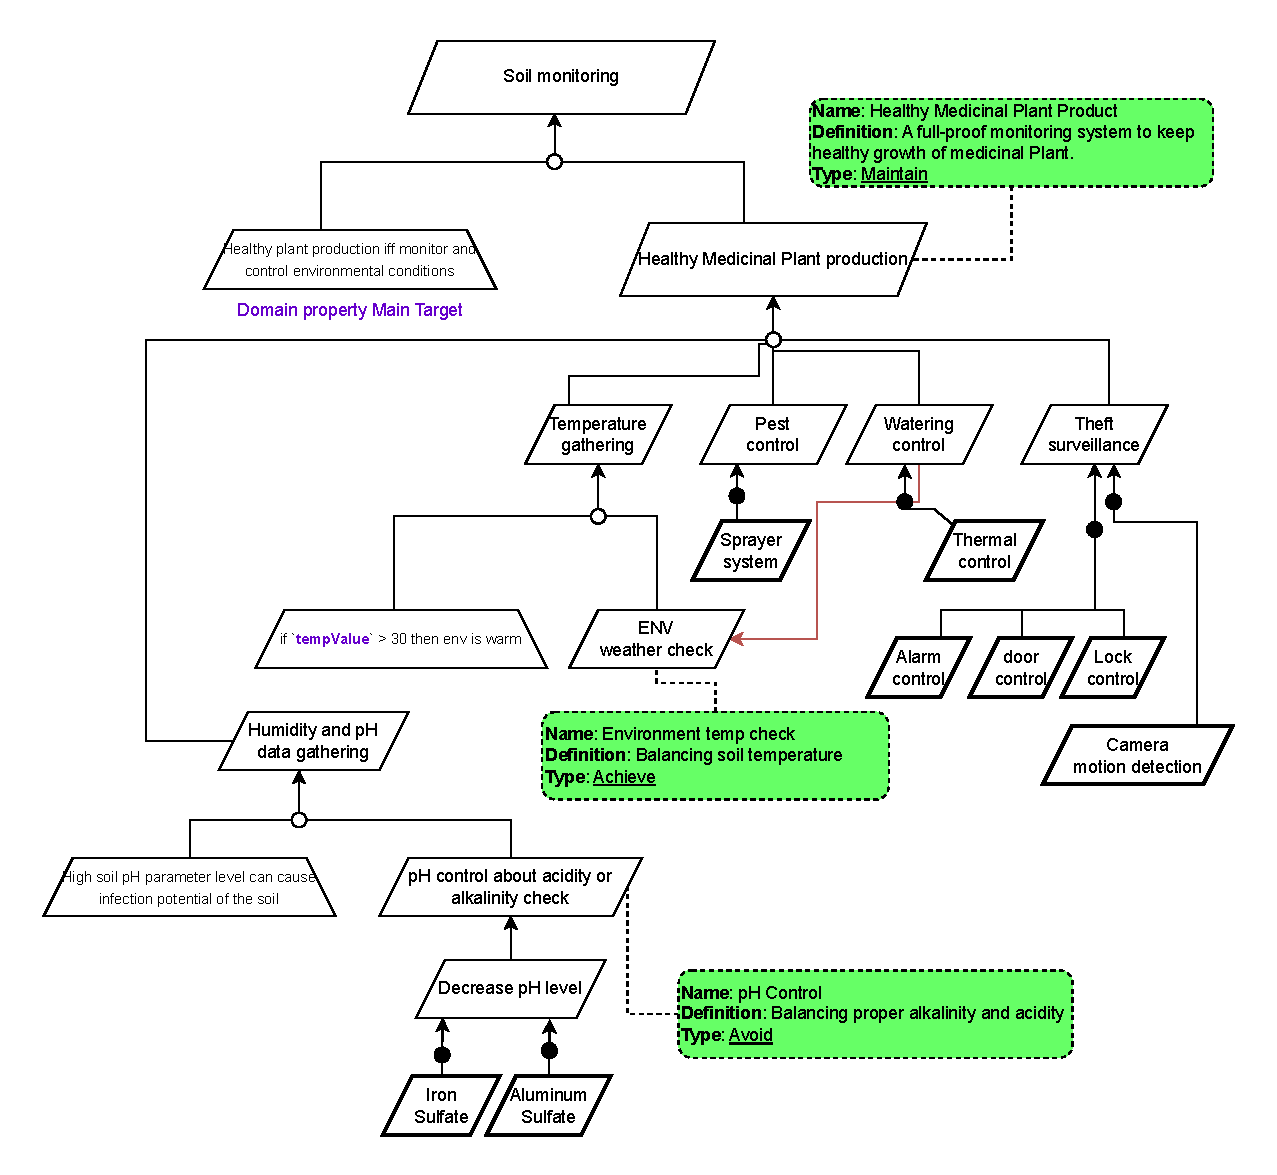
\includegraphics[width=1.0\textwidth]{assets/diagrams/soil_monitoring_goal_diagram.drawio.pdf}
    \caption{اهداف راه‌اندازی سیستم مراقبت از خاک جهت کشت گیاهان دارویی}
\end{figure}

\begin{itemize}
    \item یکی از مهم‌ترین اهداف این سیستم، کنترل سطح \lr{pH} خاک می‌باشد تا
    میزان اسیدیتی خاک را اندازه‌گیری کند و در صورت لزوم مقدار آن را کاهش دهد. دو
    راه‌کار برای این منظور در نظر گرفته شده است:
    \begin{itemize}
        \item استفاده از سولفات آهن به صورت خودکار
        \item استفاده از سولفات آلمینیوم به صورت خودکار
    \end{itemize}
    \item در این سیستم دمای محیطی به صورت مداوم پایش می‌شود و در صورتی که دما به
    بیشتر از ۳۰ درجه سانتی‌گراد رسد، میزان حرارت و دمای سیستم آبیاری نسبت با
    دمای محیط تنظیم خواهد شد و سیستم آبیاری خنک خواهد بود (با توجه به پیشنهاداتی
    که یک کشاورز می‌تواند در این زمینه فراهم کند).
    \item این سیستم باید بتواند آفات خاک و گیاهان را دفع کند برای این کار یک
    سیستم اسپری هوشمند جهت سمپاشی خاک و گیاهان بایستی راه‌اندازی شود.
    \item سیستم مورد نظر باید قابلیت‌های ضدسرقت را به همراه داشته باشد:
    \begin{itemize}
        \item با استفاده از دوربین‌های مدار بسته بتواند ضبط ۲۴ ساعته ۷ روز هفته
        داشته باشد.
        \item از سیستم کنترل قفل هوشمند استفاده کند.
        \begin{itemize}
            \item می‌تواند روی سنسور‌ها باشد.
            \item می‌تواند بر روی تمام در‌های گلخانه تنظیم و پیاده‌سازی شده باشد.
            \item یک سیستم آلارم برای اطلاع‌رسانی به افراد مشخص داشته باشد.
        \end{itemize}
    \end{itemize}
\end{itemize}

\section*{ریسک‌ها}

در این بخش به ریسک‌هایی که امکان رخ دادن آن‌ها در این سیستم محتمل است را بررسی
‌خواهیم کرد. به ازای هر سنسوری که در این سیستم مورد استفاده قرار می‌گیرد موارد
زیر در ریسک‌های سیستم دخیل خواهند بود:

\begin{itemize}
    \item امکان سوختن و از کار افتادن سنسور‌ها وجود دارد.
    \item سنسور‌ها ممکن است در برابر تغییرات آب و هوایی مقاومت مناسبی نداشته باشند.
    \item سنسور‌ها ممکن است از بین بروند و شکسته شوند:
    \begin{itemize}
        \item شکستن توسط حیوان
        \item شکستن توسط ماشین‌ها
    \end{itemize}
    \item سنسور‌ها ممکن است به سرقت بروند:
    \begin{itemize}
        \item سرقت توسط انسان
        \item سرقت توسط حیوانات
    \end{itemize}
    \item مشکلات زیرساختی و ماهیتی از سمت تجهیزات:
    \begin{itemize}
        \item مشکلات شبکه‌ای
        \item مشکلات کابل‌کشی بین \lr{Coordinator}ها و حتی سرور‌ها
        \item از بین رفتن نگهداری ظرفیت باطری سنسور
        \item مشکلات نرم‌افزار در حال اجرا در سنسور
        \item کار نکردن سنسور
        \item مشکلات سخت‌افزاری سنسور‌ها
        \item متصل نبودن سنسور
    \end{itemize}
    \item تاخیر در ارسال و اجماع داده‌ها به دلیل مصرف کمتر انرژی
    \item عدم کنترل هزینه پیاده‌سازی زیرساخت و سنسور‌ها
\end{itemize}

\begin{figure}[H]
    \centering
    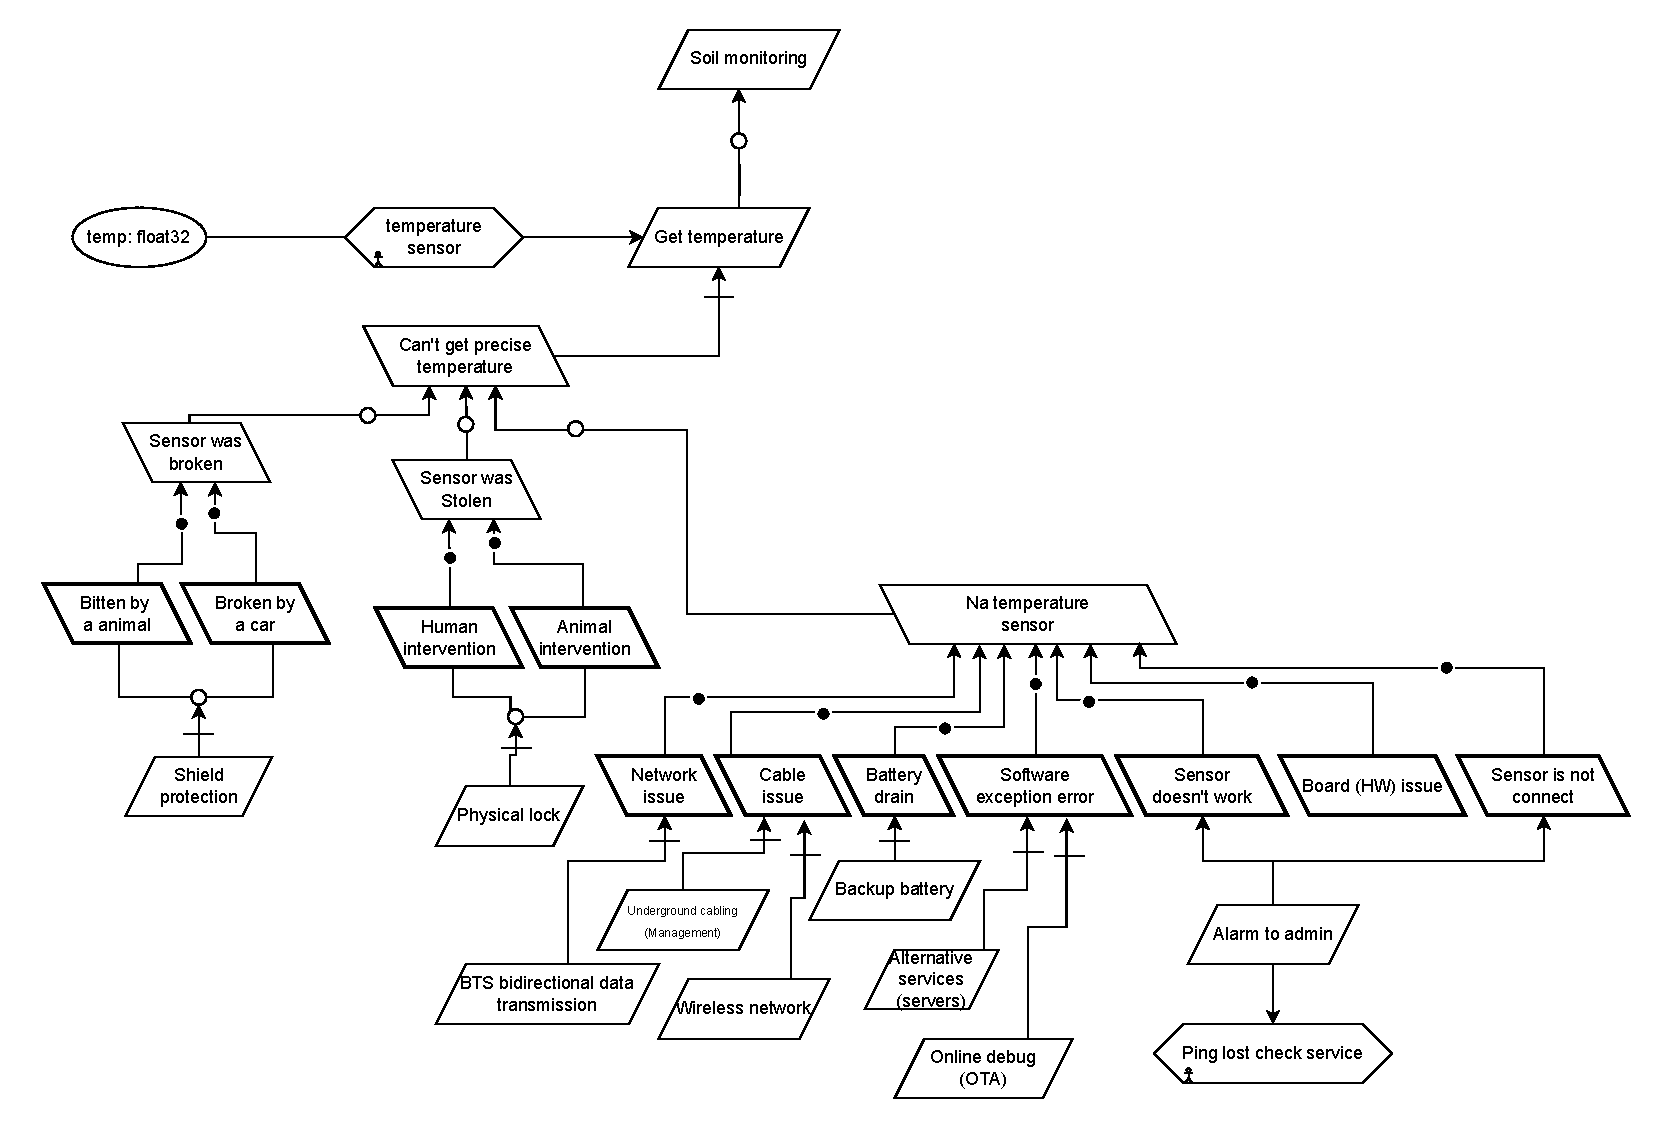
\includegraphics[width=1.0\textwidth]{assets/diagrams/risk_soil_monitoring.drawio.pdf}
    \caption{ریسک‌هایی که در برابر سنسور‌های اندازه‌گیر دما وجود دارد.}
\end{figure}

همانطور که در نمودار ریسک بالا مشاهده می‌کنید برای ریسک‌های مهم و حیاتی این
سیستم راه‌حل‌هایی را اندیشه کردیم:

\begin{itemize}
    \item برای جلوگیری از سرقت سنسور‌ها می‌توان آن‌ها را به قفل‌های هوشمند مجهز
    کرد (در شکل شماره \ref{fig:sensorTheftContextDiagram} می‌توانید نمودار مورد
    نظر را مشاهده کنید).
    \item جهت جلوگیری از شکسته شدن سنسور‌ها می‌توان برای آن‌ها قاب‌های محافظی
    طراحی کرد که آن‌ها را در برابر عوامل خارجی (به غیر از اسیدی شدن توسط خاک و
    حل شدن و اکسید شدن سنسور) مقاوم می‌سازد.
    \item مشکلات شبکه‌ای: استفاده از نحوه ارتباطی \lr{BTS} برای ارتباط دو طرفه
    جهت تبادل اطلاعات.
    \item مشکلات کابل‌کشی
    \begin{itemize}
        \item استفاده از شبکه‌های بی‌سیم
        \item استفاده از کابل‌کشی‌های زیر زمینی
    \end{itemize}
    \item زمانی که باطری سنسور به مشکل خورده باشد می‌توان سنسور‌ها را به گونه‌ای
    طراحی کرد که با باطری پشتیبان عمر آن‌ها را بیشتر کرد و بتوانیم میزان ریسک
    آن‌ها را در از کار افتادن کاهش دهیم.
    \item زمانی که نرم‌افزار موجود در سنسور‌ها به خطا‌های منطقی برخورد کند و
    باعث ایجاد \lr{Exception} شود می‌توانیم دو راه‌حل را برای کم کردن احتمال
    ریسک انجام دهیم:
    \begin{itemize}
        \item استفاده از سرویس‌های جایگزین که می‌توانند بین نرم‌افزار‌های مختلف
        در زمان وجود خطا سویچ کنند.
        \item در حین خطا‌هایی که در نرم‌افزار سنسور‌ها رخ می‌دهد دسترسی به
        سنسور‌ها را برای توسعه‌دهندگان ایجاد کنیم که بتوانند به روز رسانی‌های
        \lr{On The Air} را روی سنسور مورد نظر اعمال کنند و نرم‌افزار آن‌ها را
        رفع باگ کنند.
    \end{itemize}
    \item درصورت کار نکردن سنسور، بر اساس سرویس \lr{Ping lost check} می‌توانیم
    اطلاعات سنسور مورد نظر را در گزارش‌ها ذخیره کنیم که در چه زمانی کار نکرده و
    اتصال خود را با شبکه از دست داده‌اند. به این صورت می‌توانیم با ارائه این
    گزارش‌ها به ادمین سیستم، وی را از مشکل اتصال سنسور باخبر کنیم.
\end{itemize}

\section*{زنجیره آسیب در برابر هدف سنسور \lr{pH}}

\begin{figure}[H]
    \centering
    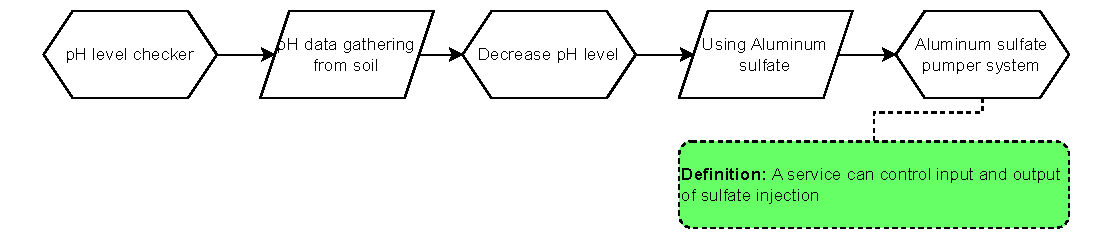
\includegraphics[width=1.0\textwidth]{assets/diagrams/ph_damage_chain_without_img.drawio.pdf}
    \caption{جهت جلوگیری از اسیدیته شدن خاک یکسری اهداف وابسته به هم وجود دارد.}
\end{figure}

\section*{\lr{Context diagram} مربوط به سرقت تجهیزات}

\begin{figure}[H]
    \centering
    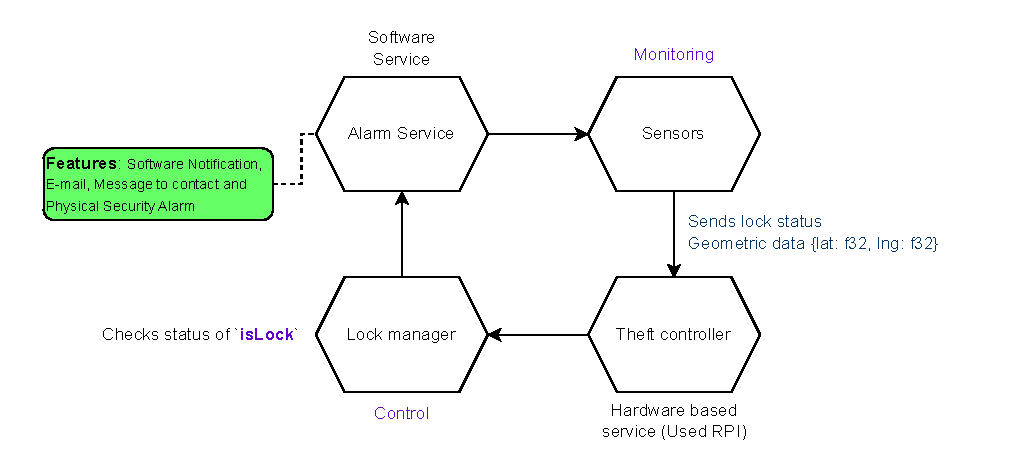
\includegraphics[width=1.0\textwidth]{assets/diagrams/sensor_theft_contex_diagram.drawio.pdf}
    \caption{عواملی که بایستی در سیستم ضد سرقت بکار گرفته شوند.}
    \label{fig:sensorTheftContextDiagram}
\end{figure}

در این دیاگرام می‌توان عملیات مانیتور و کنترل سرقت سنسور‌ها را مشاهده کرد.
سنسور‌ها را از طریق موقعیت مکانیشان (که به وسیله سنسور داخلی \lr{GPS} امکان پذیر
است) می‌توان کنترل کرد که اگر جا به جایی بیشتر از حد مجاز داشته باشند به منظور
آن است که توسط عاملی بیرونی در حال به سرقت رفتن می‌باشد. به همین خاطر اطلاعات
وضعیت قفل و مختصات جغرافیایی آن به سمت عامل کنترل سرقت ارسال می‌شود در این عامل
منطق کسب و کار بررسی می‌شود و سپس عملیات مورد نظر به سمت عامل مدیریت قفل هوشمند
ارسال می‌شود که کنترل بر سیستم هشدار مرکزی گلخانه صورت گیرد و ادمین سیستم را از
سرقت سنسور باخبر سازد.

\section*{نمودار عامل}

\begin{figure}[H]
    \centering
    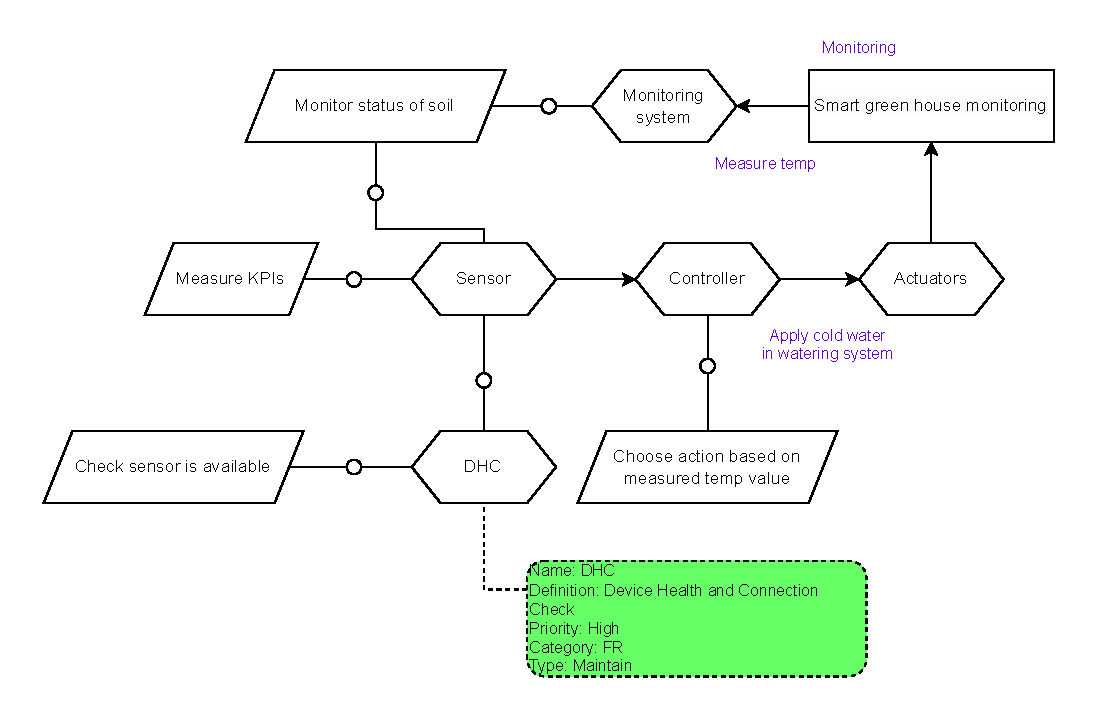
\includegraphics[width=1.0\textwidth]{assets/diagrams/agent_diagram.drawio.pdf}
    \caption{عوامل کلی که در سیستم مراقبت از خاک گلخانه هوشمند می‌توانند ایفای
    نقش کنند.}
\end{figure}

\section*{\lr{Context diagram} مربوط به سیستم هشدار آبیاری گیاهان}

\begin{figure}[H]
    \centering
    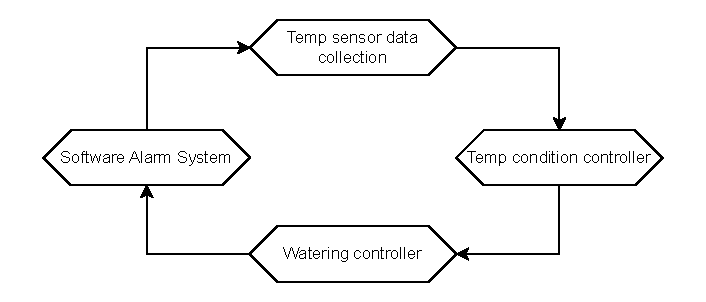
\includegraphics[width=1.0\textwidth]{assets/diagrams/temp_context_diagram.drawio.pdf}
    \caption{نمودار \lr{Context} مربوط به گرم شدن محیط و اعلام این رخداد و تغییر
    دمای سیستم آبیاری گیاهان}
\end{figure}

\section*{\lr{Class diagram}}

\begin{figure}[H]
    \centering
    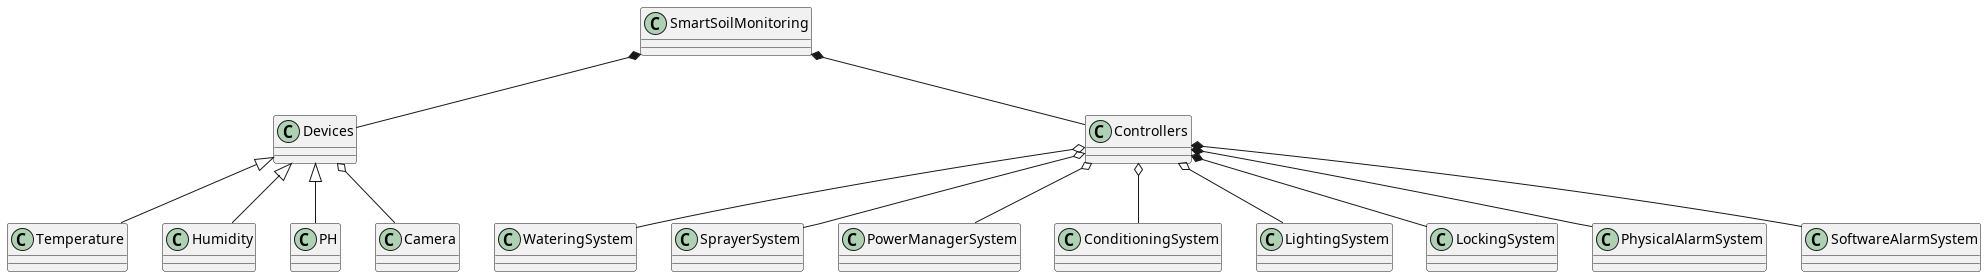
\includegraphics[width=1.0\textwidth]{assets/classes/soilMonitoring.png}
    \caption{تعیین ارتباطات بین کلاس‌ها}
\end{figure}

\begin{itemize}
    \item کلاس دستگاه‌ها و تجهیزات گلخانه حاوی ویژگی‌هایی است که کلاس‌های زیرین
    آن می‌توانند از آن ارثبری داشته باشند:
    \begin{itemize}
        \item کلاس تجهیزات اندازه‌گیر دما
        \item کلاس تجهیزات اندازه‌گیر رطوبت
        \item کلاس تجهیزات اندازه‌گیر سطح \lr{pH} خاک
        \item کلاس دوربین‌های مدار بسته که به کلاس والد خود یعنی دستگاه‌ها رابطه
        تجمیعی دارد چرا که می‌تواند به صورت مستقل از سیستم وظایف خود را انجام
        دهد.
    \end{itemize}
    \item کلاس \lr{Controllers} رابطه‌های زیر را در بر دارد:
    \begin{itemize}
        \item ارتباط تجمیعی سیستم آبیاری 
        \item ارتباط تجمیعی سیستم اسپری ضد آفت گیاهای
        \item ارتباط تجمیعی کلاس برق و انرژی گلخانه
        \item ارتباط تجمیعی کلاس سیستم تهویه هوای گلخانه
        \item ارتباط تجمیعی کلاس سیستم روشنایی
        \item ارتباط ترکیبی کلاس سیستم قفل هوشمند 
        \item ارتباط ترکیبی کلاس سیستم هشدار فیزیکی سنسور‌ها
        \item ارتباط ترکیبی کلاس سیستم هشدار نرم‌افزار جهت ایمیل، نوتیفیکیشن و
        تماس با لیست مخاطبان مشخص شده
    \end{itemize}
\end{itemize}

\end{document}
